\chapter{Numerical domains II: Octagons}
\section{Motivation}
\begin{itemize}
\item Interval domain only captures bounds of program variables
\item Many verification tasks require relational invariants
\item E.g. Buffer overflow, Concurrency bugs, Aliasing
\item Tradeoff between complexity and expressive power
\item Asymptotic Complexity: Interval $\ll$ Pentagon $\ll$ Octagon $\ll$ Polyhedra
\item Expressive Power: Interval $\ll$ Pentagon $\ll$ Octagon $ll$ Polyhedra
\end{itemize}
\section{Basics}
\begin{itemize}
\item Cubic time complexity. 
\item Used to verify correctness of software in AirBus.
\item supports limited set of linear inequalities between program variables
\item Inequalities
\begin{itemize}
\item Binary: $\pm v_j \pm v_i \leq c, v_i \neq v_j$
\item Unary: $\pm v_i \leq d$
\item $c,d \in \mathbb{R} \cup \{\infty\}$
\item If an inequality does not exist, then its bound is $\infty$
\item inequalities limit the et of possible values taken by program variable
\item for $n$ variables there are $2n^2$ possible inequalities
\end{itemize}
\item octagon can be represented by more than one set of inequalites (e.g. $(x \leq 4) \wedge (y \leq 6)$ or $(x \leq 4) \wedge (y \leq 6) \wedge (x + y \leq 10)$)
\item galois insertions need a unique representation of octagons
\item the set with maximum inequalities representing an octagon is unique. See Closure \ref{octagon_closure}
\end{itemize}

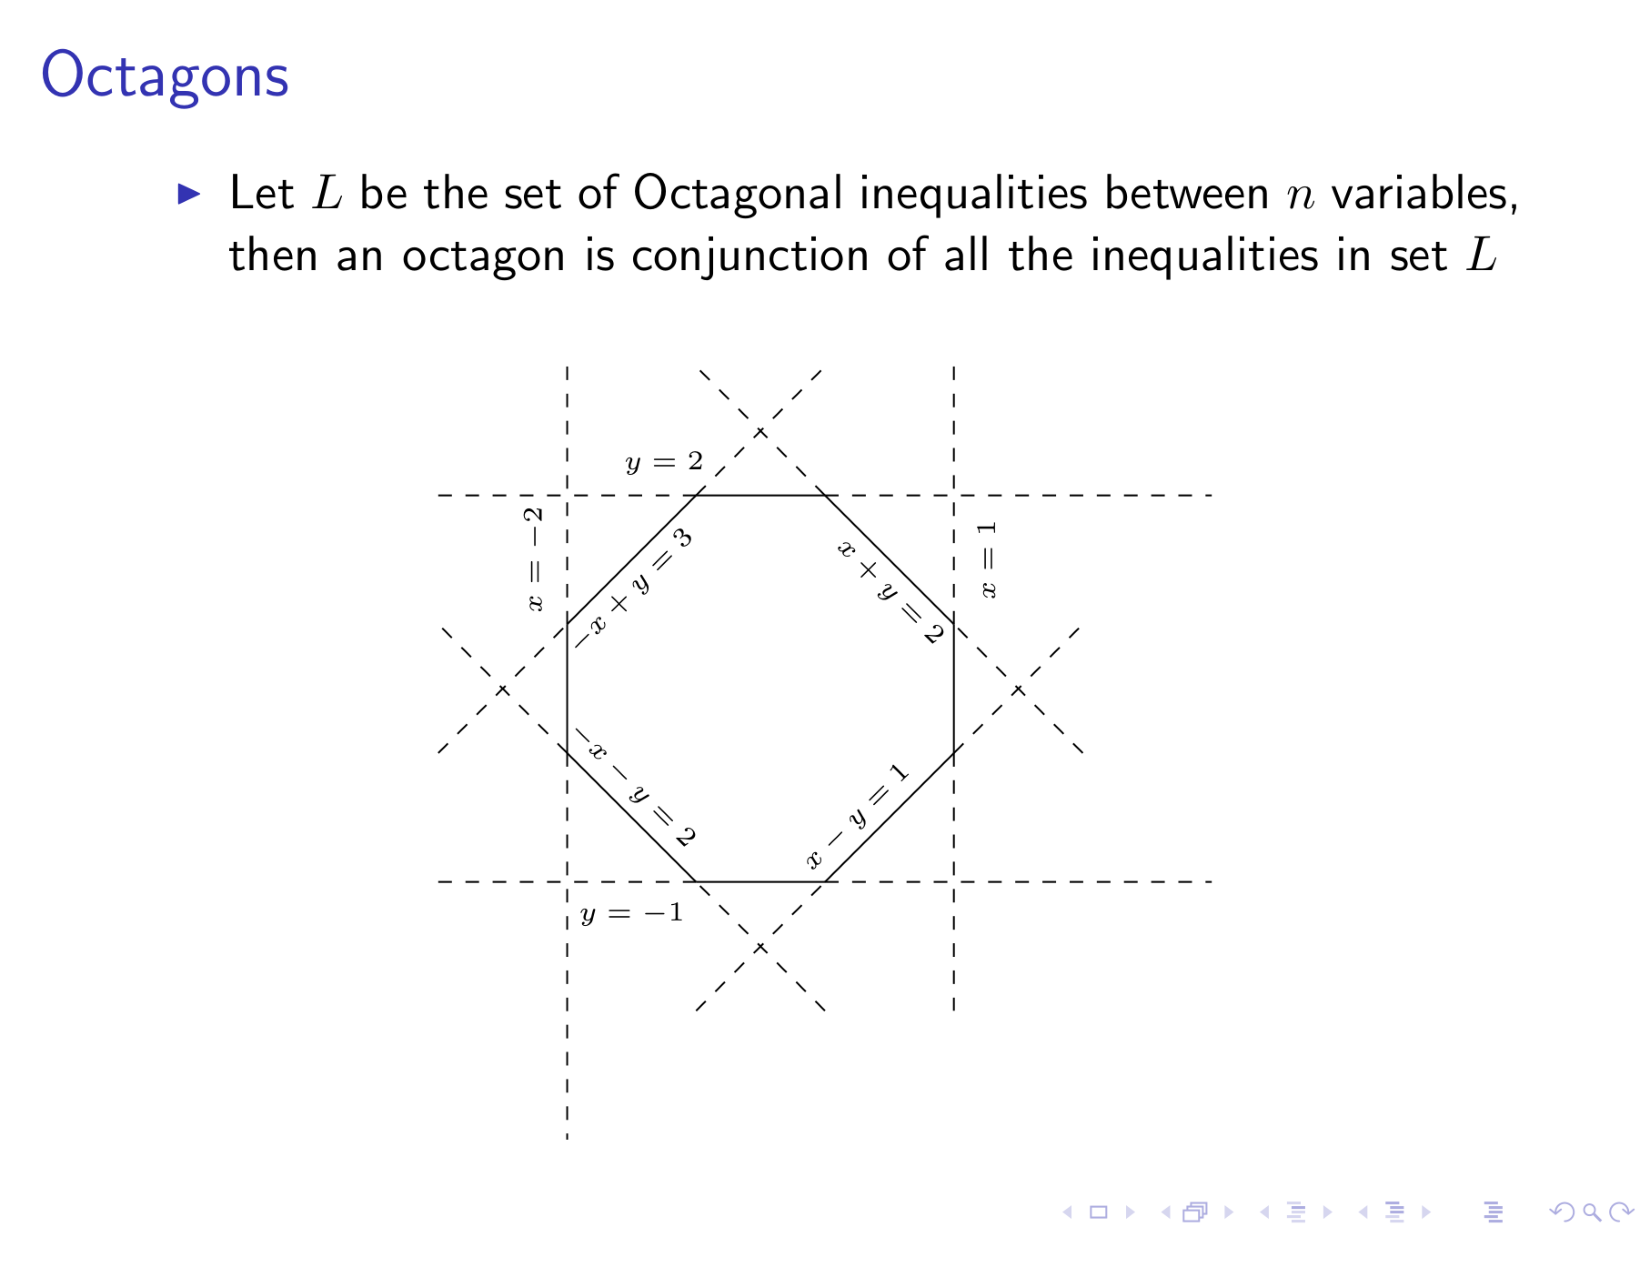
\includepdf[pages={-},nup=1x2, landscape=true]{pages/octagon.pdf}

\section{Encoding}
Matrix $m$ encodes the inequalities. For $k$ Variables $m$ has size $2k \times 2k$. Each $v_i$ is unfolded into $v'_{2i}=v_i^+$ and $v'_{2i+1}=v_i^-$.\\
$m_{i,j}=c$ represents $v'_j -v'_i \leq c$\\
$v_i + v_j \leq c$ can be represented as
\begin{itemize}
\item $v^+_j - v^-_i \leq c$\\
or
\item $v^+_i - v^-_j \leq c$
\end{itemize}
$diag(M)=0$ obviously.
\section{Formalization}
\begin{itemize}
\item The Octagon domain: $(O^O, \sqsubseteq_O, \sqcup_O, \sqcap_O, \bot_O, \top_O)$
\item $\bot_O$ represents bottom element that contains an unsatisfiable set of inequalities.
\item $O$ is the set of all octagons
\item $O^O=O \cup \{\bot_O\}$
\item $T_O$ top element for which the bound for all inequalities is $\infty$
\end{itemize}
\section{Closure(*)}
\label{octagon_closure}
The closure operator produces a unique octagon representation. Binary inequalities such as $v_i - v_j \leq c_1$ and $v_j - v_k \leq c_2$ are comined to obtain $v_i - v_k \leq c_1 + c_2$. If the octagon already contains $v_i - v_k \leq c$ then keep $v_i - v_k \leq min(c, c_1+c_2)$. (This is same as applying Floyd Warshall on the octagon matrix). The set produced by this is maximal and unique.
\section{Least Upper Bound ($\sqcup_O$)}
Union of two octagons is not necessarily an octagon. $\sqcup$ is therefore an approximation. \\
First apply closure to both operands. Then compute union by taking piecewise maximum of bounds of corresponding inequalities. \\
$(x\leq 5) \wedge (x+y \leq 10) \sqcup_O (x\leq 4) \wedge (x+y\leq 11) = (x\leq 5) \wedge (x+y \leq 11)$
\section{Geatest Lower Bound ($\sqcap_O$)}
Intersection of two octagons is always an octagon. Take piecewise minimum of bounds to calculate $\sqcap_O$.
\section{Order ($\sqsubseteq_O$)}
An octagon $O_1$ is included inside another octagon $O_2$ iff the bounds of each inequality in $O_1$ is $\leq$ than the corresponding inequality in $O_2$. Inclusion relation is used for octagon ordering. The closed octagon is the smallest octagon as per $\sqsubseteq_O$ among the set of octagons abstracting the same concrete values.
\section{Widening ($\nabla_O$)}
Widening requires the first operand to not be closed. Widening increases the number of inequalities with $\infty$ whereas closure doeas the reverse. To widen just set the bound to $\infty$ if it increases.
\section{Transformers}
\subsection{Assignment}
Transformer is precise for octagonal assignments but only approximate for those non octagonal.\\
\textbf{Octagonal assignments:}
\begin{itemize}
\item $x=c$ \\
Add inequalities $(x \leq c)$ and $(-x \leq c)$ to the octagon and \underline{close} it.
\item $x = x + c$\\
Subtract $c$ from inequalities having negative coefficient for $x$. Add $c$ to inequalities having positive coefficient for x. The result \underline{is already closed}. 
\item $x = y + c$\\
Add inequalities $(x-y\leq c)$ and $(y-x \leq c)$ to the octagon and \underline{close} it.
\end{itemize}
\textbf{Non-octagonal Assignments:}
$x_j = e$ where $x_j - e$ is non octagonal. 
\begin{enumerate}
\item Compute bounds $[a,b]$ for $e$ using interval arithmetic\\
E.g $e = [a_0, b_0] + \sum_{i=0}^n[a_i,b_i]x_i$ where each $x_i$ has bounds $[c_i,d_i]$ then $[a,b]=[a_0,b_0]+\sum_{i=1}^n[a_i,b_i] \times [c_i,d_i]$
\item Add constraints of the form $\pm x_i \pm x_j \leq [a,b] \pm [c_i,d_i]$ to the octagon.
\item close the octagon
\end{enumerate}
\subsection{Conditional Statements}
Conditional statements encode constraints which can be added to the input octagon. There are octagonal and non octagonal constraints. Similar to assignment octagonal constraints are precise whereas the other constraints are approximated.
\section{Example}
\textbf{See page 24}